%!TEX TS-program = xelatex


%%%%%%%%%%%
% General %
%%%%%%%%%%%
\documentclass[A4,11pt]{article}
\NeedsTeXFormat{LaTeX2e}
\ProcessOptions\relax
\RequirePackage[left=1.5cm,top=1.5cm,right=1.5cm,bottom=1cm,nohead,nofoot]{geometry}


%%%%%%%%%%
% Colors %
%%%%%%%%%%
\RequirePackage{xcolor}
\definecolor{white}{RGB}{255,255,255}
\definecolor{darkgray}{HTML}{333333}
\definecolor{gray}{HTML}{4D4D4D}
\definecolor{lightgray}{HTML}{999999}
\definecolor{green}{HTML}{3F913F}
\definecolor{orange}{HTML}{FDA333}
\definecolor{purple}{HTML}{3C30B1}
\definecolor{red}{HTML}{FB4485}
\definecolor{pblue}{HTML}{0395DE}
\colorlet{fillheader}{white}
\colorlet{header}{gray}
\colorlet{textcolor}{gray}
\colorlet{headercolor}{gray}


%%%%%%%%%
% Fonts %
%%%%%%%%%
\RequirePackage[quiet]{fontspec}
\RequirePackage[math-style=TeX]{unicode-math}
\newfontfamily\bodyfont
[BoldFont=texgyreheros-bold.otf,
ItalicFont=texgyreheros-italic.otf,
BoldItalicFont=texgyreheros-bolditalic.otf]
{texgyreheros-regular.otf}
\newfontfamily\thinfont[]{Lato-Light.ttf}
\newfontfamily\headingfont[]{texgyreheros-bold.otf}
\defaultfontfeatures{Mapping=tex-text}
\setmainfont
[
  Mapping=tex-text, Color=textcolor,
  BoldFont=texgyreheros-bold.otf,
  ItalicFont=texgyreheros-italic.otf,
  BoldItalicFont=texgyreheros-bolditalic.otf
]
{texgyreheros-regular.otf}
\setmathfont{texgyreheros-regular.otf}


%%%%%%%%%%%%%
% Structure %
%%%%%%%%%%%%%
\RequirePackage{parskip}
\newcounter{colorCounter}
\def\@sectioncolor#1#2#3{%
  {%
    \color{%
      \ifcase\value{colorCounter}%
        pblue\or%
        pblue\or%
        pblue\or%
        pblue\or%
        pblue\else%
        pblue\fi%
    } #1#2#3%
  }%
  \stepcounter{colorCounter}%
}
\renewcommand{\section}[1]{
  \par\vspace{\parskip}
  {
    \LARGE\headingfont\color{headercolor}%
    \@sectioncolor #1%
  }
  \par\vspace{-1.2mm}
}
\renewcommand{\subsection}[2]{
  \par\vspace{.5\parskip}%
  \Large\headingfont\color{headercolor} #2%
  \par\vspace{.25\parskip}%
}
\pagestyle{empty}


%%%%%%%%%%%%%
% Section   %
%%%%%%%%%%%%%
\setlength{\tabcolsep}{0pt}
\newenvironment{entrylist}{%
  \begin{tabular*}{\textwidth}{@{\extracolsep{\fill}}ll}
}{%
  \end{tabular*}
}
\renewcommand{\bfseries}{\headingfont\color{headercolor}}
\newcommand{\entry}[4]{
{
  \footnotesize #1}&\parbox[t]{16.0cm}{
    \textbf{#2} \\
    {\footnotesize\addfontfeature{Color=pblue} #3} \\
    {\footnotesize #4}\vspace{\parsep}
  } \\
}


%%%%%%%%%%%%%%%%%%%%
% Imports          %
%%%%%%%%%%%%%%%%%%%%
\usepackage{afterpage}
\usepackage{hyperref}
\usepackage{color}
\usepackage{xcolor}
\usepackage{graphicx}
\RequirePackage{tikz}
\hypersetup {
    pdftitle={},
    pdfauthor={},
    pdfsubject={},
    pdfkeywords={},
    colorlinks=false,
    allbordercolors=white
}


%%%%%%%%%%%%%%%%%%%%
% Document         %
%%%%%%%%%%%%%%%%%%%%
\begin{document}
\begin{minipage}[c]{0cm}
  \-\
\end{minipage}
\begin{minipage}[c]{0.2\textwidth}
  \begin{tikzpicture}
    \clip (0,0) circle (1.75cm);
    \node at (0.0, -0.7) {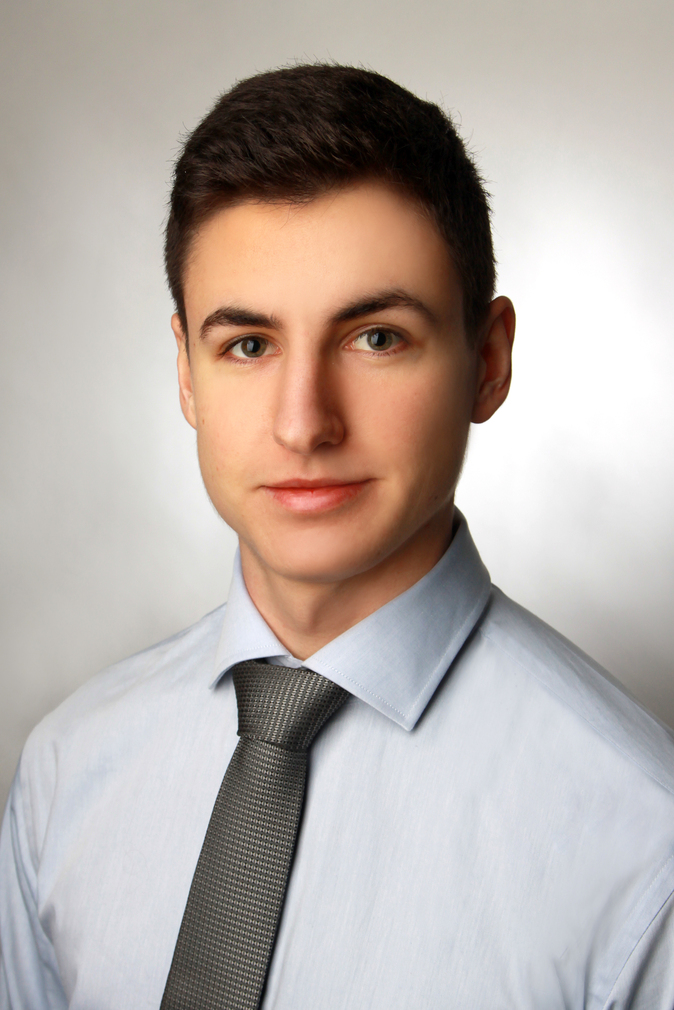
\includegraphics[width = 3.6cm]{diploma2}};    % (x, y) and width=zoom
  \end{tikzpicture}
  \hfill\vline\hfill
\end{minipage}
\begin{minipage}[c]{0.35\textwidth}
  {
    \fontsize{30pt}{62pt}\color{header}
    {\thinfont Tomasz}  {\bodyfont Kulik}
  }
  \textbf{phone:} +48 660 718 720 \\
  \href{mailto:}{\textbf{tomek.kulik2@}gmail.com} \\
  \href{https://linkedin.com/in/tomkulik}{\textbf{linkedin.com}/in/tomkulik} \\
  \href{https://github.com/kulikthebird}{\textbf{github.com}/kulikthebird} \\
\end{minipage}

\fcolorbox{white}{gray}{\parbox{\dimexpr\textwidth-2\fboxsep-2\fboxrule}{.....}}


\section{Experience}
\vspace{0.2cm}
\begin{entrylist}
  \entry
  {Jun/20 - }
  {Software Developer}
  {Luxoft (Metaswitch), Wrocław, Poland}
  {
    Some text here
    \begin{itemize}
      \setlength\itemsep{0.2em}
      \item Developing the 5G core software
      \item Implementing mainly new features
      \item Preparing the documentation and specification of the new features
      \item Working on microservices in a cloud environment (\textbf{Azure})
      \item Testing new features
      \item Working with \textbf{Docker}, \textbf{Kubernetes}
      \item Programming: \textbf{Rust}, \textbf{Python3}
    \end{itemize}
  }
  \entry
  {Aug/18 - Jun/20}
  {Engineer Software Developer}
  {Nokia, Wrocław, Poland}
  {
    After getting more experience in the project and programming skills I decided
    to focus more on the software development. Besides Python3, I started
    writing code for the telecommunication embedded system in C++14. I was
    also responsible for writing tests in TTCN-3 language. There was
    also other projects written mainly in Python in which I took part.
    \begin{itemize}
      \setlength\itemsep{0.2em}
      \item Developing of \textbf{LTE} and \textbf{IoT} software in eNodeB
      \item Developing middleware for Radio Module (\textbf{init}, \textbf{systemd})
      \item Implementing new features and maintaining legacy code
      \item Bug fixing, fault analysis
      \item Python3 and C++14 code reviewer
      \item Member of a \textbf{scrum team}
      \item Programming: \textbf{C++14}, \textbf{Python3}, \textbf{TTCN-3}, \textbf{VBA}
    \end{itemize}
  }
  \entry
  {Jun/15 - Aug/18}
  {Software Test Engineer}
  {Nokia, Wrocław, Poland}
  {
    I have started as a Working Student in Nokia by the end of a 2nd year of studies.
    I was part of Q\&A team that worked on tests for base station. After few months I
    switched to the full time job and became a Test Engineer. To get a wider view of
    the project I took part in the review process as a code reviewer. The job gave
    me a chance of working close to the 'bear metal' and simultaneously to learn
    good practices in programming. 
    \begin{itemize}
      \setlength\itemsep{0.2em}
      \item Writing \textbf{automated tests}, preparing documentation of test plans
      \item Functional Testing, Integration Testing
      \item Working on a test environment for \textbf{LTE software} U-plane and C-plane in eNodeB
      \item Python3 code review and co-author of ,,test guide''
      \item Member of a \textbf{scrum team}
      \item Programming: \textbf{Python3}, \textbf{RobotFramework}, \textbf{Bash}
    \end{itemize}
  }
\end{entrylist}

\newpage

\section{Education}
\vspace{0.1cm}
{\footnotesize
My studies were focused mainly on a theory of Computer Science, though there were also practical exercises.
I was using a number of programming languages during labs. I learned about algorithms used in various
fields such as networking, distributed systems, coding and compression of data, compilers, machine learning,
optimization and so forth.
}

\begin{entrylist}
  \entry
  {2017 - 2019}
  {Master's Degree in Computer Science (Algorithmics)}
  {Wrocław University of Science and Technology}
  {
    \emph{Faculty:} Fundamental Problems of Technology \\
    \emph{Thesis: ,,Filtering algorithms in constraints programming''.} \\
    \emph{Description and implementation of algorithms for domains reduction
      (constraints propagation) within IBM CPLEX environment. \textbf{C++11 / Optimization} }
  }
  \entry
  {2013 - 2017}
  {Bachelor's Degree in Computer Science}
  {Wrocław University of Science and Technology}
  {
    \emph{Faculty:} Fundamental Problems of Technology \\
    \emph{Thesis: ,,Computer modeling and solving geometry puzzles that require collision detection''.} \\
    \emph{Solver of 'Snake cube puzzle'. Application consist of an interactive 3D GUI that allows the user
      to manipulate the model and to solve it step by step. \textbf{C++11 / OpenGL} }
  }
\end{entrylist}


\section{Certifications}
\begin{itemize}
  \setlength\itemsep{-0.32em}
  \item {\small Best practices of object-oriented programming in C++ language}
  \item {\small ISTQB Certified Tester Foundation Level}
  \item {\small E-UTRAN/LTE Signalling}
  \item {\small LTE Cellular IoT}
\end{itemize}


\section{Tools}
\begin{itemize}
  \setlength\itemsep{-0.32em}
  \item \textbf{Cloud/DevOps:} Azure, Docker, Jenkins, Kubernetes
  \item \textbf{Programming:} Bison, Cplex, GTest, OpenGL, PyTest
  \item \textbf{Codebase and CI:} Fisheye, Gerrit, Git, Gitlab, Jenkins, Svn
  \item \textbf{Machine Learning:} Keras, Matplotlib, Pandas, Scikit-learn
  \item \textbf{Operating Systems:} Linux, Windows
  \item \textbf{Misc:} Jira, Confluence, etc.
\end{itemize}


\section{Skills}
\begin{itemize}
  \setlength\itemsep{-0.32em}
  \item \textbf{Languages:} Polish (Native), English (B2)
  \item \textbf{Programming:} C/C++ (Good), Python (Good), Rust (Intermediate),
            Julia (Intermediate), Prolog (Basic), SQL (Basic)
  \item \textbf{Personal:} Team player, Fast learner, Sharing knowledge
\end{itemize}


\section{Interested in}
\begin{itemize}
  \setlength\itemsep{-0.32em}
  \item Dance and Sport in general (trecking, snowboard, workout, etc.)
  \item Machine learning and Algorithmics
  \item Guitar
\end{itemize}


{\tiny 
  I agree to the processing of personal data provided in this document for realising
  the recruitment process pursuant to the Personal Data Protection Act of 10 May 2018 (Journal of
  Laws 2018, item 1000) and in agreement with Regulation (EU) 2016/679 of the European Parliament
  and of the Council of 27 April 2016 on the protection of natural persons with regard to the
  processing of personal data and on the free movement of such data, and repealing Directive 95/46/EC
  (General Data Protection Regulation).
}

\end{document}
